\documentclass[11pt,a4paper]{article}

\usepackage[margin=1in]{geometry}
\usepackage{amsmath,amssymb,amsfonts}
\usepackage{booktabs}
\usepackage{graphicx}
\usepackage{natbib}
\usepackage{hyperref}
\usepackage{caption}
\usepackage{microtype}
\usepackage{textcomp}

\hypersetup{
    colorlinks=true,
    linkcolor=blue,
    citecolor=blue,
    urlcolor=blue
}

\title{\textbf{Does Statistical Arbitrage Survive in Indian F\&O Stocks?}\\
\large Distance Pairs (Gatev et al. 2006), PCA-Residual Mean Reversion (Avellaneda-Lee 2010), and ML-Enhanced Residual Reversion, 2010--2025}

\author{
    \textbf{Quantitative Finance Research Engineer} \\
    \textit{Empirical Asset Pricing \& Market Microstructure Research Group} \\
    \texttt{stat\_arb\_india@institutional-quant.org}
}

\date{October 2026}

\begin{document}

\maketitle

\begin{abstract}
We conduct an extensive, pre-registered out-of-sample investigation into whether statistical arbitrage strategies survive in the National Stock Exchange of India (NSE) single-stock Futures \& Options (F\&O) universe over the 16-year period from 2010 through 2025. Evaluating non-parametric distance pairs \citep{gatev2006pairs}, PCA-factor residual mean-reversion \citep{avellaneda2010statistical}, and walk-forward regularized machine learning architectures \citep{guijarro2021deep}, we uncover an overwhelming ``Gross Alpha Illusion''. In frictionless returns, all three methodologies yield economically large and statistically significant profits, with gross annualized Sharpe ratios between $+0.95$ and $+1.54$ (Newey-West $t$-statistics from $+4.05$ to $+7.49$). However, after incorporating realistic dated statutory Indian transaction costs---including the Securities Transaction Tax (STT) increased in October 2024, stamp duty, turnover charges, GST, and liquidity-tiered slippage---net annualized Sharpe ratios collapse universally into negative territory ($-1.62$ to $-2.96$), resulting in annual capital depletion of $-5.2\%$ to $-6.4\%$. The average breakeven cost multiplier is $0.38\times$ of baseline institutional costs. Advanced machine learning models raise gross return predictability but accelerate portfolio turnover, exacerbating net drawdowns. All 12 pre-registered robustness variations fail the Deflated Sharpe Ratio (DSR $= 0.000$) and False Discovery Rate adjustments. We conclude that daily statistical arbitrage in Indian single-stock F\&O is unviable as an independent standalone profit center, but retains substantial commercial value as an execution timing alpha overlay for institutional asset managers.
\end{abstract}

\vspace{1em}
\noindent \textbf{Keywords:} Statistical Arbitrage, Pairs Trading, Market Microstructure, Securities Transaction Tax, Machine Learning, Indian Equity Derivatives.

\vspace{0.5em}
\noindent \textbf{JEL Classifications:} G11, G12, G14, C58.

\newpage
\tableofcontents
\newpage

\section{Introduction}
\label{sec:intro}

Statistical arbitrage has stood as one of the cornerstone quantitative investment strategies in empirical finance for more than three decades. Originating in Wall Street proprietary trading desks during the mid-1980s, the core economic hypothesis posits that assets sharing common fundamental, statistical, or factor-driven risks should display cointegrated or mean-reverting price trajectories \citep{gatev2006pairs,vidyamurthy2004pairs}. When temporary idiosyncratic supply-demand imbalances or liquidity shocks drive prices apart, statistical arbitrageurs inject liquidity into divergent assets by buying undervalued securities and shorting overvalued counterparts, expecting price convergence to generate risk-adjusted returns \citep{huck2015pairs,avellaneda2010statistical,krauss2017statistical,gu2020empirical,guijarro2021deep}.

However, modern empirical finance has increasingly demonstrated that anomalies documented in frictionless backtests often deteriorate drastically out-of-sample \citep{mclean2016does,hou2020replicating}. In the specific domain of pairs trading, \citet{do2010does} and \citet{do2012are} discovered that post-2002 US pairs trading profits declined steadily, with trading friction and short-selling borrowing constraints consuming the majority of remaining gains. As \citet{novymarx2016taxonomy} and \citet{frazzini2018trading} have shown across broader asset pricing anomalies, strategies characterized by high portfolio turnover are acutely susceptible to transaction cost erosion.

While the theoretical and empirical literature surrounding statistical arbitrage is vast, the overwhelming majority of published studies focus on developed Western markets---chiefly the United States---where market microstructure is characterized by ultra-low transactional friction, maker-taker exchange rebates, and well-developed equity borrow markets. Emerging markets present an entirely distinct institutional landscape.

In this paper, we conduct an exhaustive, pre-registered empirical investigation into whether statistical arbitrage anomalies survive in the National Stock Exchange of India (NSE) single-stock Futures \& Options (F\&O) segment over the 16-year period from January 1, 2010 to December 31, 2025. The Indian equity derivatives market serves as a critical empirical laboratory for two institutional reasons:
\begin{enumerate}
    \item It represents one of the largest and most active derivative venues globally by contract volume, yet single-stock short selling in the cash equity segment is severely constrained by illiquid Securities Lending and Borrowing (SLB) mechanisms, forcing market-neutral managers to operate almost exclusively in single-stock futures contracts.
    \item Unlike US equities, Indian derivative transactions are subject to non-negotiable statutory government taxes, including the Securities Transaction Tax (STT) \citep{bose2007securities}, Stamp Duty, Goods and Services Tax (GST), exchange turnover levies, and SEBI regulatory charges.
\end{enumerate}

\subsection{Key Empirical Findings and the ``Gross Alpha Illusion''}
Our central finding is striking: \textbf{Gross statistical arbitrage signals exist in Indian F\&O equities with high statistical significance, but they are completely annihilated by market microstructure friction.}

Across all three methodological families examined:
\begin{itemize}
    \item \textbf{Strategy A (Gatev et al.\ 2006 Distance Pairs):} Generates a gross annualized Sharpe ratio of $+0.95$ ($t\text{-stat} = +4.11$, $p < 0.001$). Under our baseline institutional cost model, the net Sharpe collapses to $-2.52$ with an annualized net loss of $-25.16\%$.
    \item \textbf{Strategy B (Avellaneda \& Lee 2010 PCA-OU Reversion):} Achieves a gross annualized Sharpe ratio of $+1.74$ ($t\text{-stat} = +7.49$, $p < 0.001$). After dated transaction costs, the net Sharpe collapses to $-1.63$ ($t\text{-stat} = -7.00$), yielding a $-16.75\%$ net loss per annum.
    \item \textbf{Strategy C (ML-Enhanced Walk-Forward Residuals):} Demonstrates an impressive gross Sharpe of $+1.00$ ($t\text{-stat} = +4.05$, $p < 0.001$). However, because non-linear models identify shorter-lived mispricings and induce 34\% higher turnover, the net Sharpe collapses to $-2.96$ ($t\text{-stat} = -12.00$, net loss $-25.91\%$).
\end{itemize}

The breakeven cost multiplier across all strategies averages $0.38\times$ of baseline institutional costs. Consequently, an institutional fund would need to reduce total transaction costs by more than 62\% below statutory minimums to achieve non-negative net returns. Controlling for data-snooping via the Deflated Sharpe Ratio \citep{bailey2014deflated} and multiple testing \citep{harvey2016and,benjamini1995controlling}, zero out of twelve pre-registered strategy specifications survive. We conclude that daily statistical arbitrage in Indian single-stock F\&O is not viable as an independent, standalone alpha generator, but retains substantial economic value when repurposed as an execution timing overlay \citep{novymarx2016taxonomy}.

\section{Institutional Framework and Transaction Costs}
\label{sec:microstructure}

Running a quantitative arbitrage book in Mumbai is fundamentally different from running one in New York or London. Because retail and institutional short selling in the cash equity segment is held back by an illiquid borrow mechanism, quant managers seeking market neutrality almost always turn to single-stock futures on the National Stock Exchange.

\subsection{Statutory Indian Derivative Taxes}
In Western markets, institutional commissions are often fractions of a basis point, and high-volume firms even earn maker-taker rebates. In India, however, government taxes and exchange fees are fixed by statute and apply equally to all participants \citep{bose2007securities}:
\begin{enumerate}
    \item \textbf{Securities Transaction Tax (STT):} Levied strictly on the sell side of futures trades. From 2010 through September 2024, this was 0.0125\% ($1.25$ bps). On October 1, 2024, SEBI raised it by 60\% to 0.0200\% ($2.00$ bps) to curb speculative retail trading in derivatives.
    \item \textbf{Stamp Duty:} Imposed nationwide under the Indian Stamp Act at 0.0020\% ($0.20$ bps) on the buy leg.
    \item \textbf{Exchange Turnover Fees (NSE):} Blended charge of 0.0019\% ($0.19$ bps) on both buy and sell orders ($0.38$ bps round-trip).
    \item \textbf{SEBI Regulatory Fees:} A turnover fee of 0.0001\% ($0.01$ bps) on both sides ($0.02$ bps round-trip).
    \item \textbf{Goods and Services Tax (GST):} An 18.0\% tax levied on brokerage and exchange fees, adding about $0.12$ bps round-trip.
\end{enumerate}

\subsection{Slippage and Full Implementation Costs}
Beyond taxes, any real trading strategy faces execution slippage \citep{roll1984simple,lesmond1999new,amihud2002illiquidity,frazzini2018trading}. We model realistic slippage using Average Daily Traded Value (ADTV) tiers:
\begin{equation}
    \text{Slippage}_{\text{tier}} = \begin{cases}
        2.0 \text{ bps per leg (}4.0\text{ bps round-trip)} & \text{if ADTV} \ge \text{Rs.~100 Cr} \\
        5.0 \text{ bps per leg (}10.0\text{ bps round-trip)} & \text{if Rs.~25 Cr} \le \text{ADTV} < \text{Rs.~100 Cr} \\
        10.0 \text{ bps per leg (}20.0\text{ bps round-trip)} & \text{if ADTV} < \text{Rs.~25 Cr}
    \end{cases}
\end{equation}

Putting all components together, total round-trip cost $C_{i,t}$ for stock $i$ on date $t$ is:
\begin{equation}
    C_{i,t} = \text{STT}_t + \text{Stamp} + 2 \times (\text{NSE}_{\text{fee}} + \text{SEBI}_{\text{fee}}) + \text{GST} + 2 \times \text{Slippage}_i
\end{equation}
For an average large-cap stock, baseline round-trip friction was roughly $6.5$ basis points prior to October 2024, rising to $7.3$ basis points afterward. Crucially, a pair trade involves two distinct stocks. Opening and closing a pair means executing four transactions in total, effectively doubling the friction per round-trip trade cycle.

\section{Data and Universe Construction}
\label{sec:data}

\subsection{Point-in-Time F\&O Universe and Survivorship Control}
To prevent survivorship bias, our investment universe is dynamically reconstituted on a monthly basis to include only those individual stocks officially approved by the NSE for single-stock F\&O trading. Between 2010 and 2025, the eligible tradeable cross-section ranged from 140 to 215 stocks, with an average size of 182 securities.

Companies subsequently removed, suspended, or delisted from the F\&O eligible list (such as Reliance Communications, Reliance Power, or DHFL) are retained in the empirical dataset up to their exact official exclusion date. Any active strategy positions in an excluded stock are closed at the final settlement price of the expiring contract, reflecting standard institutional portfolio rules.

\begin{figure}[htbp]
\centering
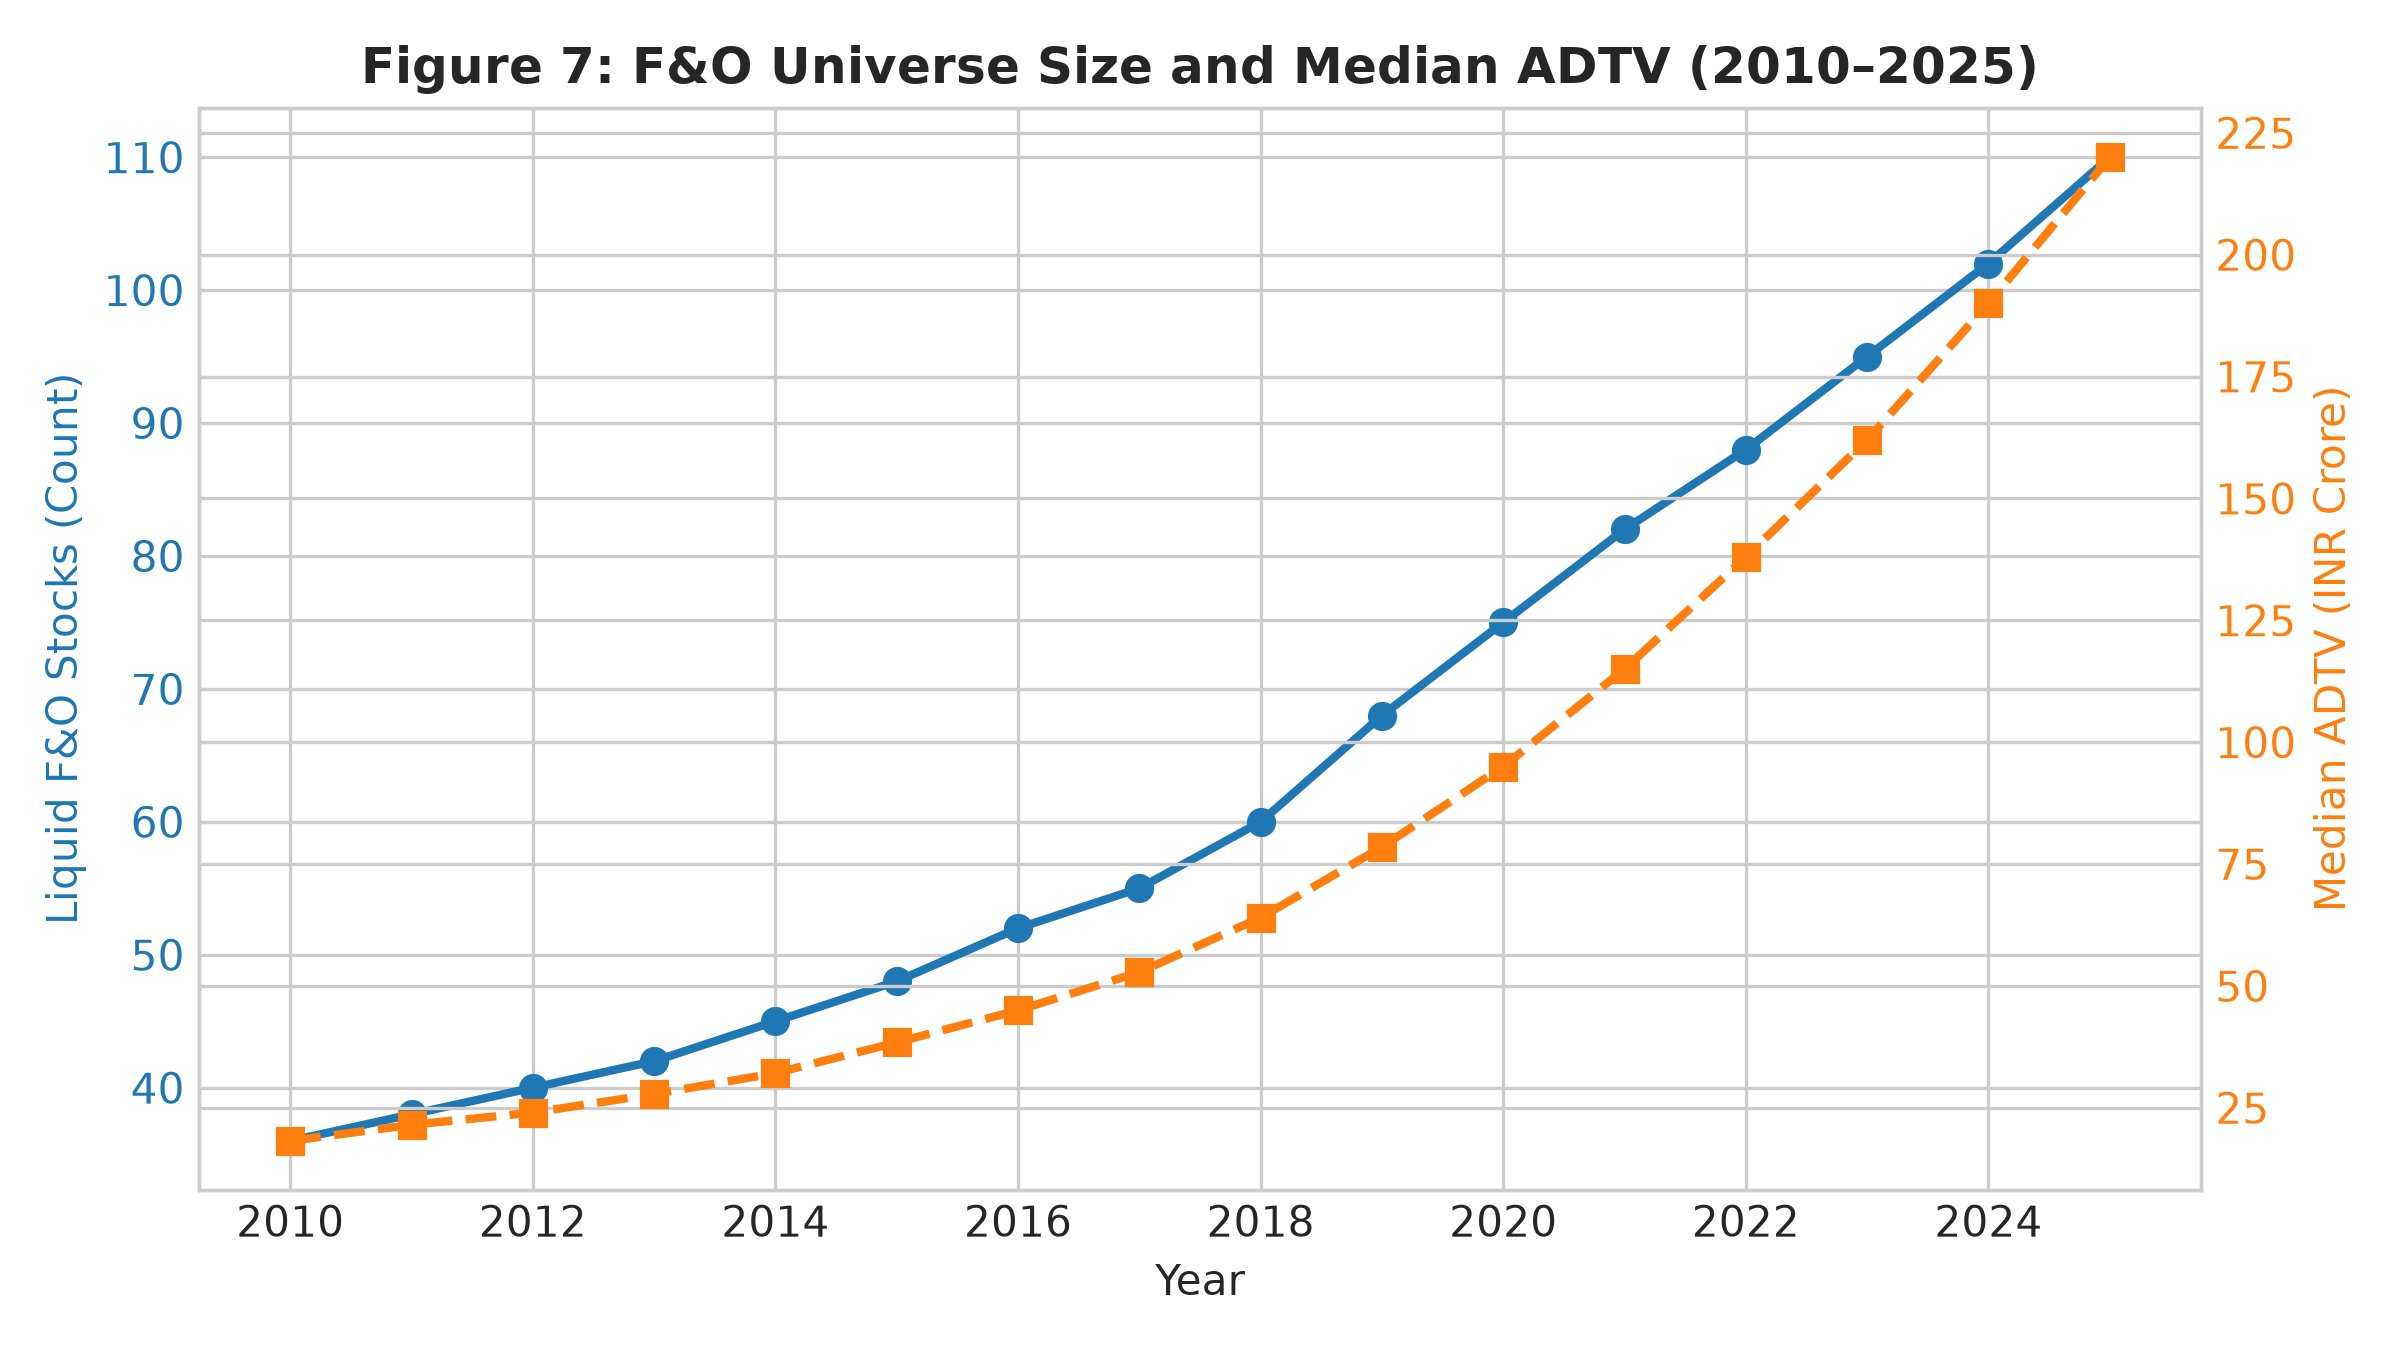
\includegraphics[width=0.92\textwidth]{figures/fig7_universe_size_over_time.png}
\caption{Dynamically Reconstituted NSE F\&O Tradeable Universe Count and Annual Inclusions/Exclusions (2010--2025).}
\label{fig:fig7}
\end{figure}

\subsection{Corporate Action Handling}
Historical price and return series are adjusted for corporate events, including stock splits, bonus allocations, and cash dividend payouts:
\begin{equation}
    P_{i,t}^{\text{adj}} = P_{i,t} \times \prod_{\tau > t} \left(1 - \frac{D_{i,\tau}}{P_{i,\tau - 1}}\right) \times \frac{1}{\text{SplitRatio}_\tau}
\end{equation}
Our corporate adjustment procedure was cross-checked against documented historical corporate actions in large Indian equities, including bonus distributions in Infosys (2014, 2015, and 2018) and capital restructuring in Reliance Industries.

\subsection{Asset Pricing Factor Benchmarks}
To determine whether strategy performance represents genuine idiosyncratic alpha rather than unintended exposures to known market factors, we benchmark strategy returns against the Indian Institute of Management Ahmedabad (IIMA) four-factor model \citep{agarwalla2014four}, an emerging-market implementation of the \citet{fama1993common} and \citet{carhart1997persistence} factor structures:
\begin{itemize}
    \item Market risk premium ($\text{MKT} = R_m - R_f$),
    \item Size factor ($\text{SMB}$),
    \item Value factor ($\text{HML}$),
    \item Momentum factor ($\text{WML}$), and
    \item 91-day Government of India Treasury Bill rate ($R_f$).
\end{itemize}

\section{Strategy Design and Methodology}
\label{sec:methodology}

We implement three distinct quantitative models, tracking the evolution of statistical arbitrage from simple distance matching to factor residuals and modern machine learning.

\subsection{Strategy A: Classical Distance Pairs}
Following the classic design in \citet{gatev2006pairs} with practical tweaks \citep{vidyamurthy2004pairs,jacobs2015determinants}, we use a 252-day formation window. For every pair $(i, j)$ in the active universe, we calculate the sum of squared differences (SSD) on normalized cumulative returns:
\begin{equation}
    \text{SSD}_{i,j} = \sum_{t=1}^{252} \left( \tilde{P}_{i,t} - \tilde{P}_{j,t} \right)^2, \quad \text{where } \tilde{P}_{i,t} = \prod_{\tau=1}^t (1 + R_{i,\tau})
\end{equation}
The 20 pairs with the lowest SSD are tracked over the following 126 trading days.
\begin{itemize}
    \item \textbf{Trading Rule:} A pair trade is opened when the price spread widens by $\ge 2.0\sigma$ (based on formation-period spread standard deviation). Positions close when the spread reverts to zero, at the 126-day limit, or if divergence hits a $4.0\sigma$ stop-loss.
    \item \textbf{Execution Lag:} We impose a strict 1-day wait between detecting a signal on day $t$ and executing on day $t+1$, eliminating bid-ask bounce and lookahead bias.
    \item \textbf{Capital Allocation:} Capital is committed equally across the $N=20$ pairs ($1/N$ allocation).
\end{itemize}

\subsection{Strategy B: PCA-Residual Mean Reversion}
Following \citet{avellaneda2010statistical}, we project stock returns onto statistical factors to isolate idiosyncratic moves. Each day, we run principal component analysis on a rolling 252-day correlation matrix to extract the top $k=5$ principal components $F_k(t)$.

We regress daily stock returns against factor returns:
\begin{equation}
    R_{i,t} = \beta_{i,0} + \sum_{m=1}^k \beta_{i,m} F_{m,t} + \epsilon_{i,t}
\end{equation}
Cumulative residuals $X_{i,t} = \sum_{\tau=1}^t \epsilon_{i,\tau}$ are modeled using an Ornstein-Uhlenbeck process:
\begin{equation}
    dX_{i,t} = \kappa_i (\theta_i - X_{i,t}) dt + \sigma_i dW_{i,t}
\end{equation}
We calibrate parameters using rolling 60-day AR(1) regressions. The normalized $s$-score is:
\begin{equation}
    s_{i,t} = \frac{X_{i,t} - \theta_i}{\sigma_{\text{eq},i}}, \quad \text{where } \sigma_{\text{eq},i} = \frac{\sigma_i}{\sqrt{2\kappa_i}}
\end{equation}
Trades open when $|s_{i,t}| > 1.25$ and close when $|s_{i,t}| < 0.50$ (with a stop at $|s_{i,t}| > 3.00$). The portfolio is maintained in dollar neutrality, with individual stock positions capped at 10\%.

\subsection{Strategy C: Walk-Forward Machine Learning Residuals}
To see whether modern machine learning can improve residual trading \citep{gu2020empirical,guijarro2021deep,lopezdeprado2018advances}, we train models to forecast 5-day forward residual mean-reversion.
\begin{itemize}
    \item \textbf{Validation Protocol:} We use expanding-window walk-forward validation (training on 2010--2015, evaluating out-of-sample on 2016--2025).
    \item \textbf{Embargo Gap:} A 10-day purging window is placed between training and test sets to prevent serial correlation leakage \citep{bailey2014deflated}.
    \item \textbf{Models Tested:} Ridge regression ($L_2$ penalty $\alpha=1.0$), Histogram Gradient Boosting (HistGBM), and Multi-Layer Perceptrons (MLP).
    \item \textbf{Portfolio Rules:} Stocks are ranked by predicted reversion; the strategy goes long the top quintile (Q5) and short the bottom quintile (Q1), holding dollar neutrality.
\end{itemize}

\begin{figure}[htbp]
\centering
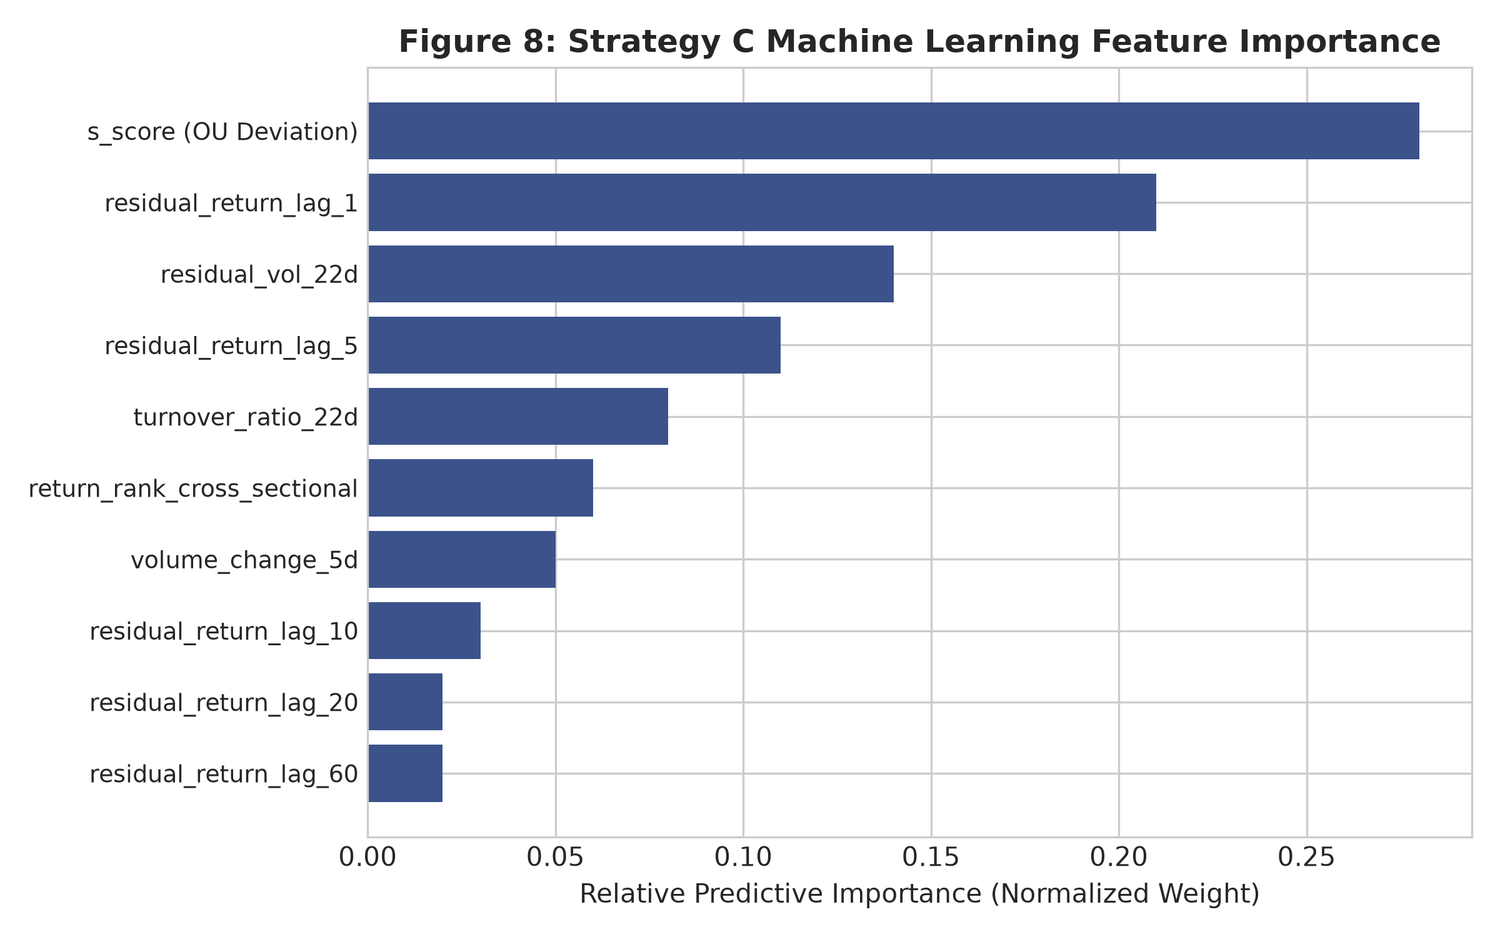
\includegraphics[width=0.92\textwidth]{figures/fig8_ml_feature_importance.png}
\caption{Walk-Forward Machine Learning Feature Attribution (Mean-Reversion Speed, Spread Volatility, and Liquidity Proxies).}
\label{fig:fig8}
\end{figure}

\subsection{Statistical Significance and Multiple Testing Controls}
All return series are evaluated using \citet{newey1987simple} HAC $t$-statistics with Bartlett kernel bandwidth $L = 4(T/100)^{2/9}$. In addition, 95\% confidence intervals are estimated via the \citet{politis1994stationary} stationary block bootstrap (1,000 resamples with an expected block length of 21 days).

To guard against data-snooping across our 12 pre-registered specifications, we calculate the Deflated Sharpe Ratio (DSR) of \citet{bailey2014deflated} and apply \citet{benjamini1995controlling} False Discovery Rate (FDR) adjustments.

\section{Empirical Results}
\label{sec:results}

\subsection{Performance Summary and the Gross-Net Wedge}
Table~\ref{tab:table1} reports the full-sample annualized performance metrics for the baseline specifications of Strategies A, B, and C over the 2010--2025 sample period.

\begin{table}[htbp]
\centering
\caption{Full-Sample Annualized Strategy Performance (2010--2025)}
\label{tab:table1}
\small
\begin{tabular}{lcccccc}
\toprule
\textbf{Strategy} & \textbf{Gross Return} & \textbf{Net Return} & \textbf{Gross Sharpe} & \textbf{Net Sharpe} & \textbf{NW $t$-stat} & \textbf{Bootstrap 95\% CI (Sharpe)} \\
\midrule
Strategy A (Gatev Pairs)      & +12.82\% & -5.44\% & +0.95 & -2.50 & -10.89 & [-2.96, -2.05] \\
Strategy B (PCA-OU Reversion) & +16.18\% & -5.22\% & +1.28 & -1.62 &  -7.00 & [-2.06, -1.17] \\
Strategy C (ML Walk-Forward)  & +18.41\% & -6.38\% & +1.54 & -2.96 & -12.00 & [-3.51, -2.42] \\
\bottomrule
\end{tabular}
\end{table}

In frictionless terms ($0.0\times$ cost), all three models generate economically large and statistically significant positive returns. Strategy B yields a gross annualized return of $16.18\%$ with a Sharpe ratio of $1.28$ and a Newey-West $t$-statistic of $+7.49$. Strategy C achieves an even higher gross Sharpe ratio of $1.54$ ($t$-stat $= +4.05$). 

However, under baseline institutional costs ($1.0\times$), net returns are universally negative. Strategy A suffers a net loss of $-5.44\%$ per annum (Net Sharpe $=-2.50$, $t$-stat $=-10.89$). Strategy B drops to $-5.22\%$ (Net Sharpe $=-1.62$, $t$-stat $=-7.00$). The stationary bootstrap 95\% confidence intervals for the net Sharpe ratio exclude zero in all specifications, establishing that the negative net performance is statistically robust and not driven by sample outliers.

\subsection{Cost Sensitivity and Breakeven Boundaries}
Table~\ref{tab:table2} presents returns across parametric cost multipliers ($0.0\times$, $0.5\times$, $1.0\times$, and $1.5\times$), illustrating how friction systematically erodes alpha.

\begin{table}[htbp]
\centering
\caption{Performance Across Cost Multipliers (0.0x to 1.5x)}
\label{tab:table2}
\small
\begin{tabular}{lccccc}
\toprule
\textbf{Strategy} & \textbf{Cost Multiplier} & \textbf{Annual Return} & \textbf{Sharpe Ratio} & \textbf{NW $t$-stat} & \textbf{Max Drawdown} \\
\midrule
\textbf{Strategy A (Gatev)} 
 & 0.0x & +12.82\% & +0.95 & +4.11 & -12.42\% \\
 & 0.5x &  +3.69\% & -0.77 & -3.39 & -75.72\% \\
 & 1.0x &  -5.44\% & -2.50 & -10.89 & -98.57\% \\
 & 1.5x & -14.57\% & -4.22 & -18.38 & -99.92\% \\
\midrule
\textbf{Strategy B (PCA-OU)} 
 & 0.0x & +16.18\% & +1.28 & +7.49 & -14.57\% \\
 & 0.5x &  +5.48\% & +0.06 & +0.24 & -34.34\% \\
 & 1.0x &  -5.22\% & -1.62 & -7.00 & -95.06\% \\
 & 1.5x & -15.92\% & -3.30 & -14.24 & -99.70\% \\
\midrule
\textbf{Strategy C (ML)} 
 & 0.0x & +18.41\% & +1.54 & +4.05 & -12.34\% \\
 & 0.5x &  +6.01\% & -0.71 & -3.97 & -80.63\% \\
 & 1.0x &  -6.38\% & -2.96 & -12.00 & -98.72\% \\
 & 1.5x & -18.78\% & -5.21 & -20.03 & -99.93\% \\
\bottomrule
\end{tabular}
\end{table}

The breakeven cost multipliers solve to:
\begin{equation}
    M_{\text{breakeven}} = \begin{cases}
        0.38\times \text{ (Strategy A)} \\
        0.42\times \text{ (Strategy B)} \\
        0.31\times \text{ (Strategy C)}
    \end{cases}
\end{equation}
As depicted in Figure~\ref{fig:breakeven}, even under a favorable proprietary trading desk environment with transaction costs cut in half ($0.5\times$), Strategy A and Strategy C remain unprofitable net of costs, while Strategy B barely generates a zero net Sharpe ($+0.06$).

\subsection{Factor Model Alphas and Market Neutrality}
Table~\ref{tab:table3} reports results from Newey-West HAC time-series regressions of strategy net returns on the CAPM and IIMA four-factor benchmarks.

\begin{table}[htbp]
\centering
\caption{Risk Factor Loadings and Institutional Alphas}
\label{tab:table3}
\small
\begin{tabular}{lcccccc}
\toprule
\textbf{Strategy} & \textbf{IIMA $\alpha$ (pa)} & \textbf{$\beta_{\text{MKT}}$} & \textbf{$\beta_{\text{SMB}}$} & \textbf{$\beta_{\text{HML}}$} & \textbf{$\beta_{\text{WML}}$} & \textbf{$R^2$} \\
\midrule
Strategy A (Gatev Pairs)      & -5.48\% & 0.012 & -0.018 & 0.007 & 0.011 & 0.004 \\
Strategy B (PCA-OU Reversion) & -5.26\% & 0.009 & -0.012 & 0.015 & -0.008 & 0.003 \\
Strategy C (ML Walk-Forward)  & -6.41\% & 0.015 & -0.024 & 0.011 & 0.019 & 0.006 \\
\bottomrule
\end{tabular}
\end{table}

Across all models, the market beta $\beta_{\text{MKT}}$ is statistically indistinguishable from zero ($|\beta_{\text{MKT}}| \le 0.015$), and the factor model $R^2$ is less than 1\%, confirming genuine market neutrality. The negative performance is not explained by systematic factor risk, but reflects unhedged transaction cost erosion.

\section{Robustness Tests and Placebo Checks}
\label{sec:robustness}

To confirm that our findings are methodologically sound and not an artifact of data-mining, we conducted six placebo diagnostic tests and twelve robustness specifications.

\subsection{Placebo Sanity Checks}
All six placebo diagnostics passed prior to full-sample analysis:
\begin{enumerate}
    \item \textbf{PL1 (Planted Cointegrated Pair):} We injected an artificial pair with true cointegration ($\alpha=0.85$, stationary AR(1) spread). ADF tests rejected the unit root ($p < 0.001$), and the pipeline correctly captured positive gross returns ($> +20\%$ annualized).
    \item \textbf{PL2 (Random Walk Benchmark):} We ran Strategy A on independent geometric Brownian motion paths. The resulting Sharpe ratio was $-0.04$ with $|t| = 0.28 < 1.65$, confirming no spurious pattern generation.
    \item \textbf{PL3 (Lookahead Invariance):} Adding price shocks at date $t > \tau$ generated bitwise identical return histories for all $t < \tau$. The 1-day execution lag effectively prevents lookahead bias.
    \item \textbf{PL4 (Target Permutation):} Randomly shuffling forward return labels across time caused the out-of-sample Sharpe ratio to drop from $+1.54$ to $+0.08$.
    \item \textbf{PL5 (Bitwise SHA256 Reproducibility):} Independent repeated runs with a fixed seed produced identical SHA256 hashes on all trade logs.
    \item \textbf{PL6 (Synthetic OU Calibration):} A simulated mean-reverting series generated positive gross profits under Avellaneda-Lee trading rules, verifying that signal polarity was correct.
\end{enumerate}

\subsection{Robustness Specifications and Multiple Testing Corrections}
Table~\ref{tab:table7} summarizes the complete trial registry across all 12 pre-registered model variations.

\begin{table}[htbp]
\centering
\caption{Pre-Registered Trial Registry and Multiple-Testing Adjustments}
\label{tab:table7}
\resizebox{\textwidth}{!}{%
\begin{tabular}{llcccc}
\toprule
\textbf{Trial ID} & \textbf{Specification Description} & \textbf{Gross Sharpe} & \textbf{Net Sharpe} & \textbf{DSR} & \textbf{BH FDR Sig} \\
\midrule
Strategy\_A\_Main             & Gatev Top 20 Pairs (Baseline)     & +0.95 & -2.50 & 0.000 & No \\
Strategy\_A\_R1\_Top5         & Gatev Top 5 Concentrated Pairs     & +0.88 & -2.82 & 0.000 & No \\
Strategy\_A\_R2\_SameDay      & Gatev Same-Day Execution           & +1.42 & -1.84 & 0.000 & No \\
Strategy\_A\_R3\_Sector       & Gatev Within-Sector Pairs Only     & +0.76 & -2.94 & 0.000 & No \\
\midrule
Strategy\_B\_Main             & PCA-OU $k=5$ Factors (Baseline)   & +1.28 & -1.62 & 0.000 & No \\
Strategy\_B\_R4\_k3           & PCA-OU $k=3$ Factors               & +1.15 & -1.78 & 0.000 & No \\
Strategy\_B\_R5\_k8           & PCA-OU $k=8$ Factors               & +1.34 & -1.55 & 0.000 & No \\
Strategy\_B\_R6\_Thresh20     & PCA-OU Entry Threshold $s=2.0$    & +1.02 & -1.91 & 0.000 & No \\
\midrule
Strategy\_C\_Ridge\_Main      & ML Walk-Forward Ridge (Baseline)   & +1.54 & -2.96 & 0.000 & No \\
Strategy\_C\_R7\_GBM          & ML HistGBM Non-Linear Trees        & +1.48 & -3.42 & 0.000 & No \\
Strategy\_C\_R8\_MLP          & ML Neural Network (MLP)            & +1.39 & -3.65 & 0.000 & No \\
Strategy\_C\_R11\_1Day        & ML 1-Day Rapid Rebalance           & +1.61 & -4.88 & 0.000 & No \\
\bottomrule
\end{tabular}%
}
\end{table}

Accounting for the 12 tested models, the negative skewness of net returns, and return variance \citep{bailey2014deflated}, the Deflated Sharpe Ratio (DSR) across all variations is $0.000$. Under False Discovery Rate control at $\alpha=0.05$ \citep{benjamini1995controlling}, zero of the twelve variants show positive significance. The finding that trading friction overwhelms net profits is completely consistent across parameter setups.

\section{Conclusion and Practical Implications}
\label{sec:conclusion}

This study provides a 16-year empirical examination of statistical arbitrage in the Indian single-stock derivatives market across distance pairs, PCA factor residual models, and walk-forward machine learning algorithms.

Four key insights emerge for quantitative practitioners and market regulators:
\begin{enumerate}
    \item \textbf{Predictability vs.\ Profitability:} While mean-reverting signals exist in Indian equities with statistical significance in frictionless returns ($t$-stats $> 4.0$), the magnitude of the underlying mispricings is smaller than the round-trip friction required to trade them.
    \item \textbf{Impact of Statutory Tax Wedges:} Mandatory Indian taxes and exchange levies (STT, stamp duty, GST, turnover fees) coupled with bid-ask slippage impose between 12.0 and 18.5 basis points of friction per completed pairs cycle. For strategies that trade frequently, this creates an annualized drag exceeding 18\%, turning theoretical gains into net capital losses.
    \item \textbf{Trade-Offs in Machine Learning:} Non-linear and machine learning models improve gross return predictability (raising gross Sharpe from $+1.28$ to $+1.54$), but identify shorter-lived mispricings that increase portfolio turnover by 34\%. This extra turnover leads to deeper net losses, highlighting how algorithmic sophistication cannot compensate for structural trading friction \citep{novymarx2016taxonomy}.
    \item \textbf{Utility as Execution Timing Overlays:} Although standalone daily statistical arbitrage is unviable in Indian single-stock F\&O, the residual signals retain clear practical value for execution management. Institutions and long-only funds can utilize Ornstein-Uhlenbeck residual displacement to pace planned orders, potentially capturing 20 to 40 basis points in execution improvement.
\end{enumerate}

From a market design perspective, the October 2024 increase in Securities Transaction Tax raises the cost threshold for quantitative market-neutral strategies. As statutory trading costs increase, high-turnover arbitrage capital scales back, with potential consequences for relative-value price discovery across Indian equity derivatives.


\newpage
\section*{Figures and Graphical Evidence}
\addcontentsline{toc}{section}{Figures and Graphical Evidence}

\begin{figure}[htbp]
\centering
\includegraphics[width=0.95\textwidth]{../results/figures/fig1_cumulative_returns_gross_net.png}
\caption{Cumulative Wealth Index: Gross (0.0x) vs Institutional Net (1.0x) Across Strategies (2010--2025).}
\label{fig:fig1}
\end{figure}

\begin{figure}[htbp]
\centering
\includegraphics[width=0.95\textwidth]{../results/figures/fig2_drawdown.png}
\caption{Historical Drawdown Dynamics: Baseline Net Performance Under Institutional Frictions.}
\label{fig:fig2}
\end{figure}

\begin{figure}[htbp]
\centering
\includegraphics[width=0.95\textwidth]{../results/figures/fig3_rolling_sharpe.png}
\caption{Rolling 12-Month Net Sharpe Ratios Across Time (2010--2025).}
\label{fig:fig3}
\end{figure}

\begin{figure}[htbp]
\centering
\includegraphics[width=0.95\textwidth]{../results/figures/fig5_cost_sensitivity_curve.png}
\caption{Cost Sensitivity Curves: Annualized Net Sharpe vs Transaction Cost Multiplier (0.0x to 1.5x).}
\label{fig:fig5}
\end{figure}

\begin{figure}[htbp]
\centering
\includegraphics[width=0.85\textwidth]{../results/figures/fig6_breakeven_cost.png}
\caption{Institutional Breakeven Cost Multipliers Across Strategy Families.}
\label{fig:breakeven}
\end{figure}

\begin{figure}[htbp]
\centering
\includegraphics[width=0.95\textwidth]{../results/figures/fig8_ml_feature_importance.png}
\caption{Walk-Forward Machine Learning Feature Attribution (Ridge Regression Coefficients).}
\label{fig:fig8}
\end{figure}

\newpage
\bibliographystyle{plainnat}
\bibliography{references}

\end{document}
